\documentclass[aspectratio=169]{../latex_main/tntbeamer}  % you can pass all options of the beamer class, e.g., 'handout' or 'aspectratio=43'
\usepackage{dsfont}
\usepackage{bm}
\usepackage[english]{babel}
\usepackage[T1]{fontenc}
%\usepackage[utf8]{inputenc}
\usepackage{graphicx}
\graphicspath{ {./figures/} }
\usepackage{algorithm}
\usepackage[ruled,vlined,algo2e,linesnumbered]{algorithm2e}
\usepackage{hyperref}
\usepackage{booktabs}
\usepackage{mathtools}

\usepackage{amsmath,amssymb}

\DeclareMathOperator*{\argmax}{arg\,max}
\DeclareMathOperator*{\argmin}{arg\,min}

\usepackage{amsbsy}
\newcommand{\vect}[1]{\bm{#1}}
%\newcommand{\vect}[1]{\boldsymbol{#1}}

\usepackage{pgfplots}
\pgfplotsset{compat=1.16}
\usepackage{tikz}
\usetikzlibrary{trees} 
\usetikzlibrary{shapes.geometric}
\usetikzlibrary{positioning,shapes,shadows,arrows,calc,mindmap}
\usetikzlibrary{positioning,fadings,through}
\usetikzlibrary{decorations.pathreplacing}
\usetikzlibrary{intersections}
\pgfdeclarelayer{background}
\pgfdeclarelayer{foreground}
\pgfsetlayers{background,main,foreground}
\tikzstyle{activity}=[rectangle, draw=black, rounded corners, text centered, text width=8em]
\tikzstyle{data}=[rectangle, draw=black, text centered, text width=8em]
\tikzstyle{myarrow}=[->, thick, draw=black]

% Define the layers to draw the diagram
\pgfdeclarelayer{background}
\pgfdeclarelayer{foreground}
\pgfsetlayers{background,main,foreground}

% Requires XeLaTeX or LuaLaTeX
%\usepackage{unicode-math}

\usepackage{fontspec}
%\setsansfont{Arial}
\setsansfont{RotisSansSerifStd}[ 
Path=../latex_main/fonts/,
Extension = .otf,
UprightFont = *-Regular,  % or *-Light
BoldFont = *-ExtraBold,  % or *-Bold
ItalicFont = *-Italic
]
\setmonofont{Cascadia Mono}[
Scale=0.8
]

% scale factor adapted; mathrm font added (Benjamin Spitschan @TNT, 2021-06-01)
%\setmathfont[Scale=1.05]{Libertinus Math}
%\setmathrm[Scale=1.05]{Libertinus Math}

% other available math fonts are (not exhaustive)
% Latin Modern Math
% XITS Math
% Libertinus Math
% Asana Math
% Fira Math
% TeX Gyre Pagella Math
% TeX Gyre Bonum Math
% TeX Gyre Schola Math
% TeX Gyre Termes Math

% Literature References
\newcommand{\lit}[2]{\href{#2}{\footnotesize\color{black!60}[#1]}}

%%% Beamer Customization
%----------------------------------------------------------------------
% (Don't) Show sections in frame header. Options: 'sections', 'sections light', empty
\setbeamertemplate{headline}{empty}

% Add header logo for normal frames
\setheaderimage{
	% 
\includegraphics[height=\logoheight]{figures/TNT_darkv4.pdf}
	
\includegraphics[height=\logoheight]{../latex_main/figures/luh_logo_rgb_0_80_155.pdf}
	% 
\includegraphics[height=\logoheight]{figures/logo_tntluh.pdf}
}

% Header logo for title page
\settitleheaderimage{
	% 
\includegraphics[height=\logoheight]{figures/TNT_darkv4.pdf}
	
\includegraphics[height=\logoheight]{../latex_main/figures/luh_logo_rgb_0_80_155.pdf}
	% 
\includegraphics[height=\logoheight]{figures/logo_tntluh.pdf}
}

% Title page: tntdefault 
\setbeamertemplate{title page}[tntdefault]  % or luhstyle
% Add optional title image here
%\addtitlepageimagedefault{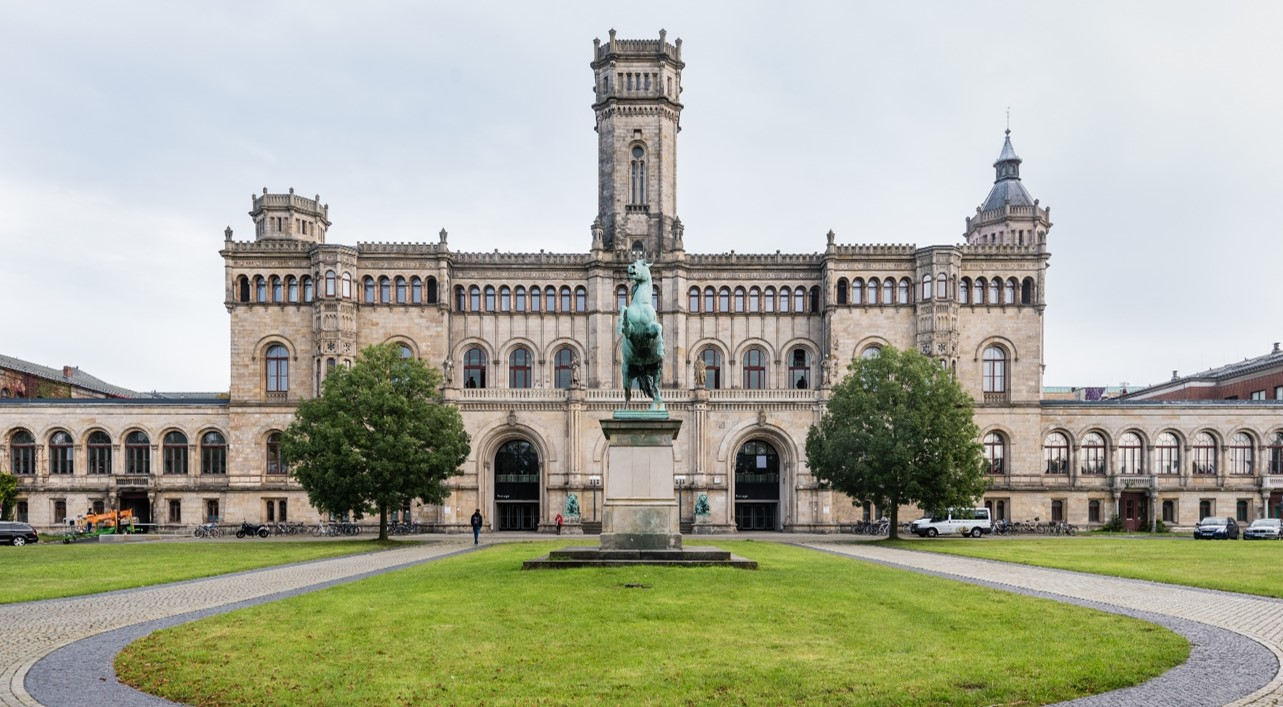
\includegraphics[width=0.65\textwidth]{figures/luh_default_presentation_title_image.jpg}}

% Title page: luhstyle
% \setbeamertemplate{title page}[luhstyle]
% % Add optional title image here
% \addtitlepageimage{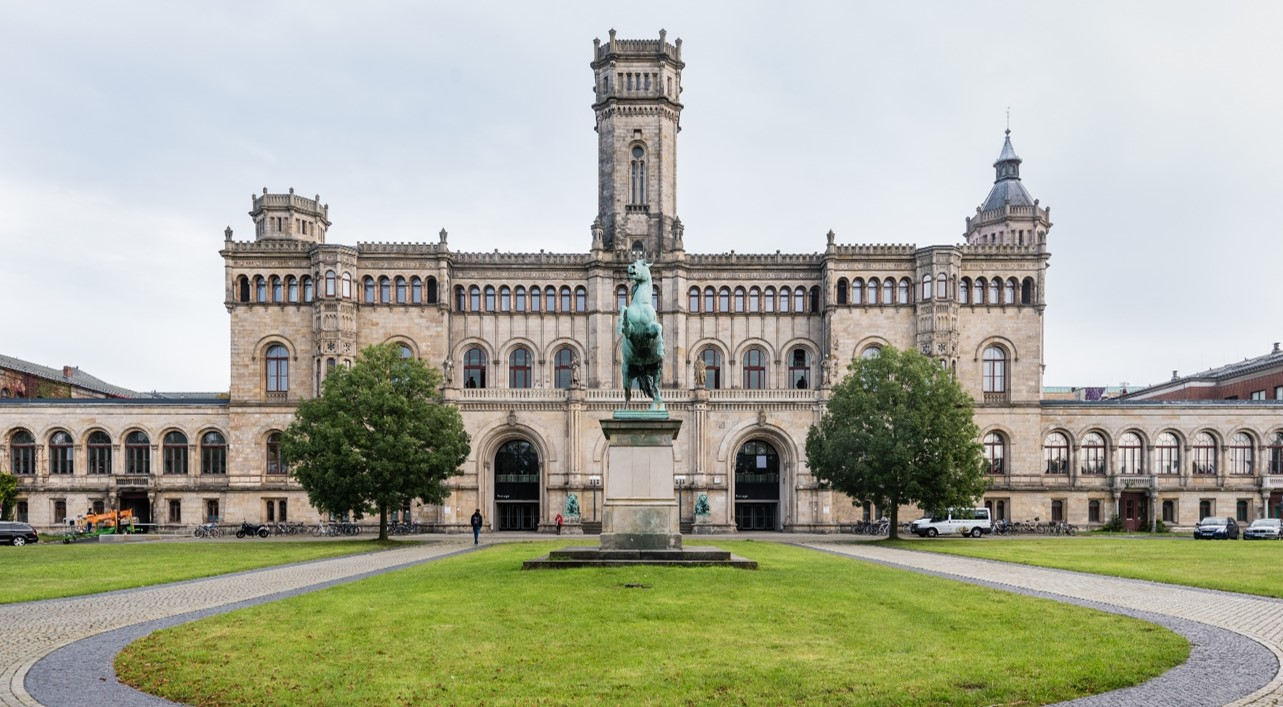
\includegraphics[width=0.75\textwidth]{figures/luh_default_presentation_title_image.jpg}}

\author[Abedjan \& Lindauer]{Ziawasch Abedjan \& Marius Lindauer\\[1em]
	
\includegraphics[height=\logoheight]{../latex_main/figures/luh_logo_rgb_0_80_155.pdf}\qquad
	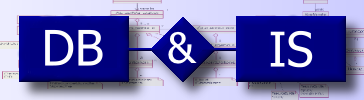
\includegraphics[height=\logoheight]{../latex_main/figures/DBIS_Kurzlogo.png}\qquad

\includegraphics[height=\logoheight]{../latex_main/figures/TNT_darkv4}\qquad

\includegraphics[height=\logoheight]{../latex_main/figures/L3S.jpg}	}
\date{Summer Term 2022; \hspace{0.5em} {
\includegraphics[height=1.5em]{../latex_main/figures/Cc-by-nc-sa_icon.svg.png}}; based on \href{https://ds100.org/fa21/}{[DS100]}
}


%%% Custom Packages
%----------------------------------------------------------------------
% Create dummy content
\usepackage{blindtext}

% Adds a frame with the current page layout. Just call \layout inside of a frame.
\usepackage{layout}


%%% Macros
%\renewcommand{\vec}[1]{\mathbf{#1}}
% \usepackage{bm}
%\let\vecb\bm

\title[Visualization]{DS: Visualization}
\subtitle{Rug plots, histograms, density curves}

\graphicspath{ {./figure/} }
%\institute{}


\begin{document}
	
	\maketitle
    \begin{frame}{Rug plot}
        \begin{columns}
            \begin{column}{.5\textwidth}
                    \begin{itemize}
                        \item Rug plots are used to show the distribution of a single quantitative (numerical) variable.
                        \item They show us each and every value!
                        \item Issues with rug plots:
                        \begin{itemize}
                            \item Too much detail.
                            \item Hard to see the bigger picture.
                            \item Overplotting.
                            \begin{itemize}
                                \item How many birth weights were at 120?
                                \item[$\leadsto$] Can’t tell – they’re all on top of each other.
                            \end{itemize}
                        \end{itemize}
                    \end{itemize}
            \end{column}
            
            
            \begin{column}{.4\textwidth}
            
                       \centering
                       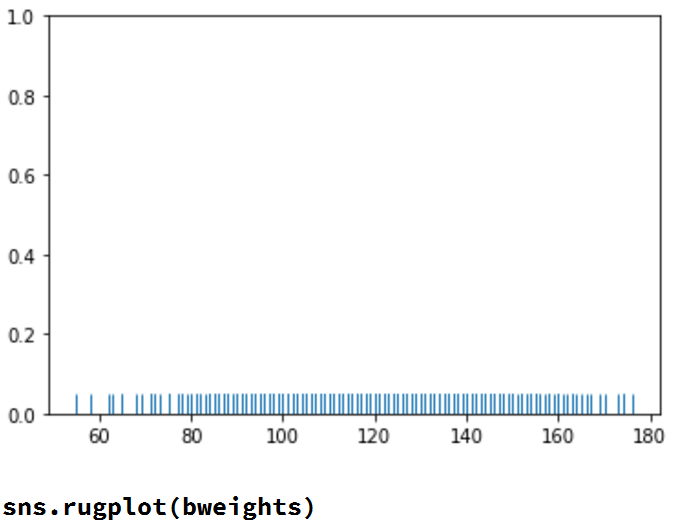
\includegraphics[scale=.35]{Bild26}
                       
            \end{column}
        \end{columns}
    \end{frame}
    
    
     \begin{frame}{Histograms}
        \begin{columns}
            \begin{column}{.6\textwidth}
                    \begin{itemize}
                        \item Histograms can be thought of as a smoothed version of a rug plot
                        \begin{itemize}
                            \item Lose granularity, but gain interpretability.
                        \end{itemize}
                        \item Horizontal axis: the number line, divided into bins.
                        \item Areas represent proportions!
                        \begin{itemize}
                            \item Total area = 1 (or 100\%).
                        \end{itemize}
                        \item Units of height: proportion per unit on the x-axis.
                        \begin{itemize}
                            \item Can be seen by dividing the above equation by “width of bin”.
                        \end{itemize}
                    \end{itemize}
            \end{column}
            
            
            \begin{column}{.4\textwidth}
            
                       \centering
                       
\includegraphics[scale=.5]{Bild27}
                       
            \end{column}
        \end{columns}
    \end{frame}
    
    
    \begin{frame}{Histograms}
        \begin{columns}
            \begin{column}{.4\textwidth}
                   By default, matplotlib histograms show counts on the y-axis, not proportions per unit. 
                   \begin{figure}
                       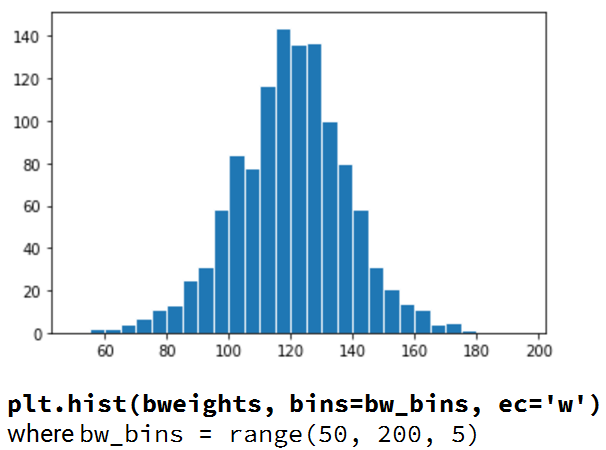
\includegraphics[scale=.35]{Bild28}
                   \end{figure}
            \end{column}
            
            
            \begin{column}{.4\textwidth}
                We use the optional density parameter to fix the y-axis. After doing this, the total area sums to 1.

                       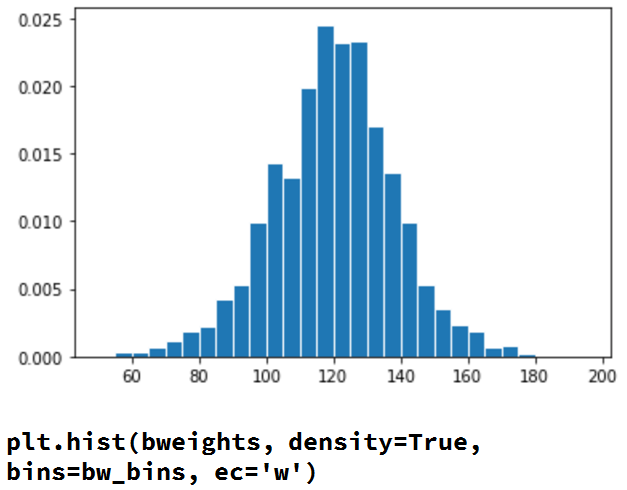
\includegraphics[scale=.35]{Bild29}

            \end{column}
        \end{columns}
    \end{frame}
    
    
    \begin{frame}[c]{Example calculation}
        \begin{columns}
            \begin{column}{.4\textwidth}
            
                   Approximately ~120 babies were born with a weight between 110 and 115.\\
                   \bigskip
                   There are 1174 observations total.

            \end{column}
            
            
            \begin{column}{.4\textwidth}
                   \begin{figure}
                       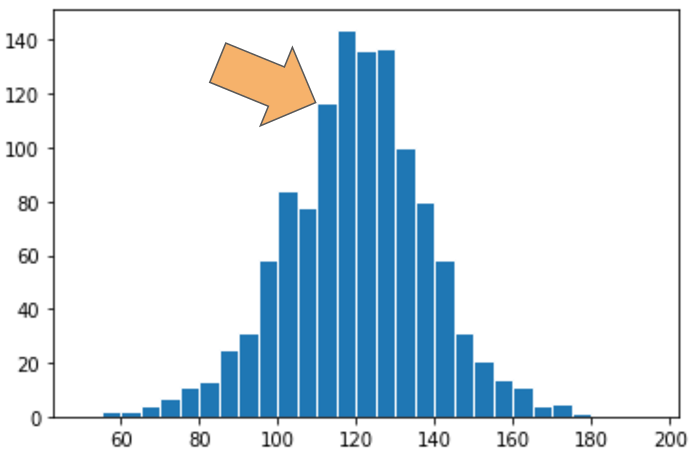
\includegraphics[scale=.35]{Bild30}
                   \end{figure}

            \end{column}
        \end{columns}
    \end{frame}
    
    
    
     \begin{frame}[c]{Example calculation}
        \begin{columns}
            \begin{column}{.4\textwidth}
                   There are 1174 observations total.\\
                   \bigskip
                    Width of bin [110, 115): 5\\
                    Height of bar [110, 115): 0.02\\
                    Proportion in bin = 5 * 0.02 = 0.1\\
                    Number in bin = 0.1 * 1174 = 117.4\\
                    \bigskip
                    This is roughly the number we got before (120)!

            \end{column}
            
            
            \begin{column}{.4\textwidth}
            
                       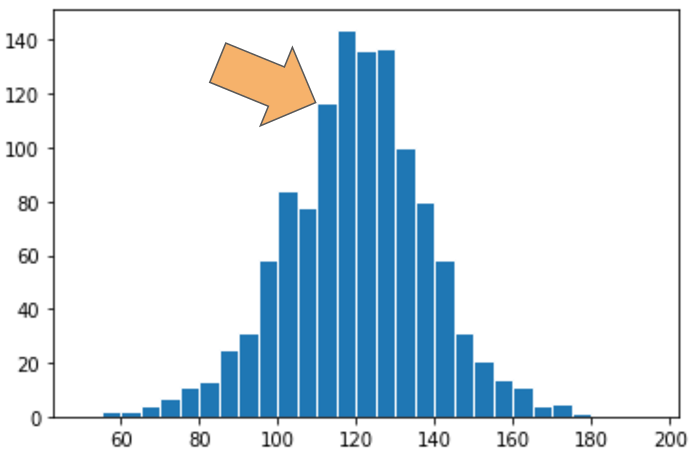
\includegraphics[scale=.35]{Bild30}

            \end{column}
        \end{columns}
    \end{frame}
    
    
    
    
    \begin{frame}{Histograms}
        \vspace{-2em}
        \begin{columns}
        
            \begin{column}{.4\textwidth}
            
                      \centering
                      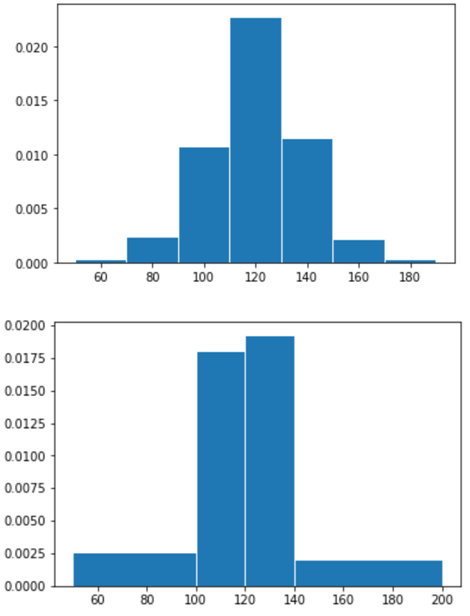
\includegraphics[scale=.35]{Bild31}

            \end{column}
            
            
            \begin{column}{.6\textwidth}
            
                  Beware of drawing strong conclusions from the looks of a histogram. The number of bins influences its appearance!\\
                  The Freedman-Diaconis rule
                  \begin{equation*}
                      \text{Bin width} = 2\dfrac{IQR(x)}{\sqrt[3]{n}}
                  \end{equation*}
                \texttt{plt.hist(bweights, bins = np.arange(50, 200, 20), density=True, ec='w')}\\
                \bigskip
                Bins don’t need to have the same width! When they don’t, it’s especially crucial to think of proportions as areas.\\
                \bigskip
                \texttt{plt.hist(bweights, bins = [50, 100, 120, 140, 200], density=True, ec='w')}

            \end{column}
        \end{columns}
    \end{frame}
    
    \begin{frame}[c]{Histogram vs. eCDF}
    
        \vspace{-3em}
        \begin{columns}
            \begin{column}{.5\textwidth}
            
                      \centering
                      Histograms with $\#$bins$=\{10,50\}$ \\
                      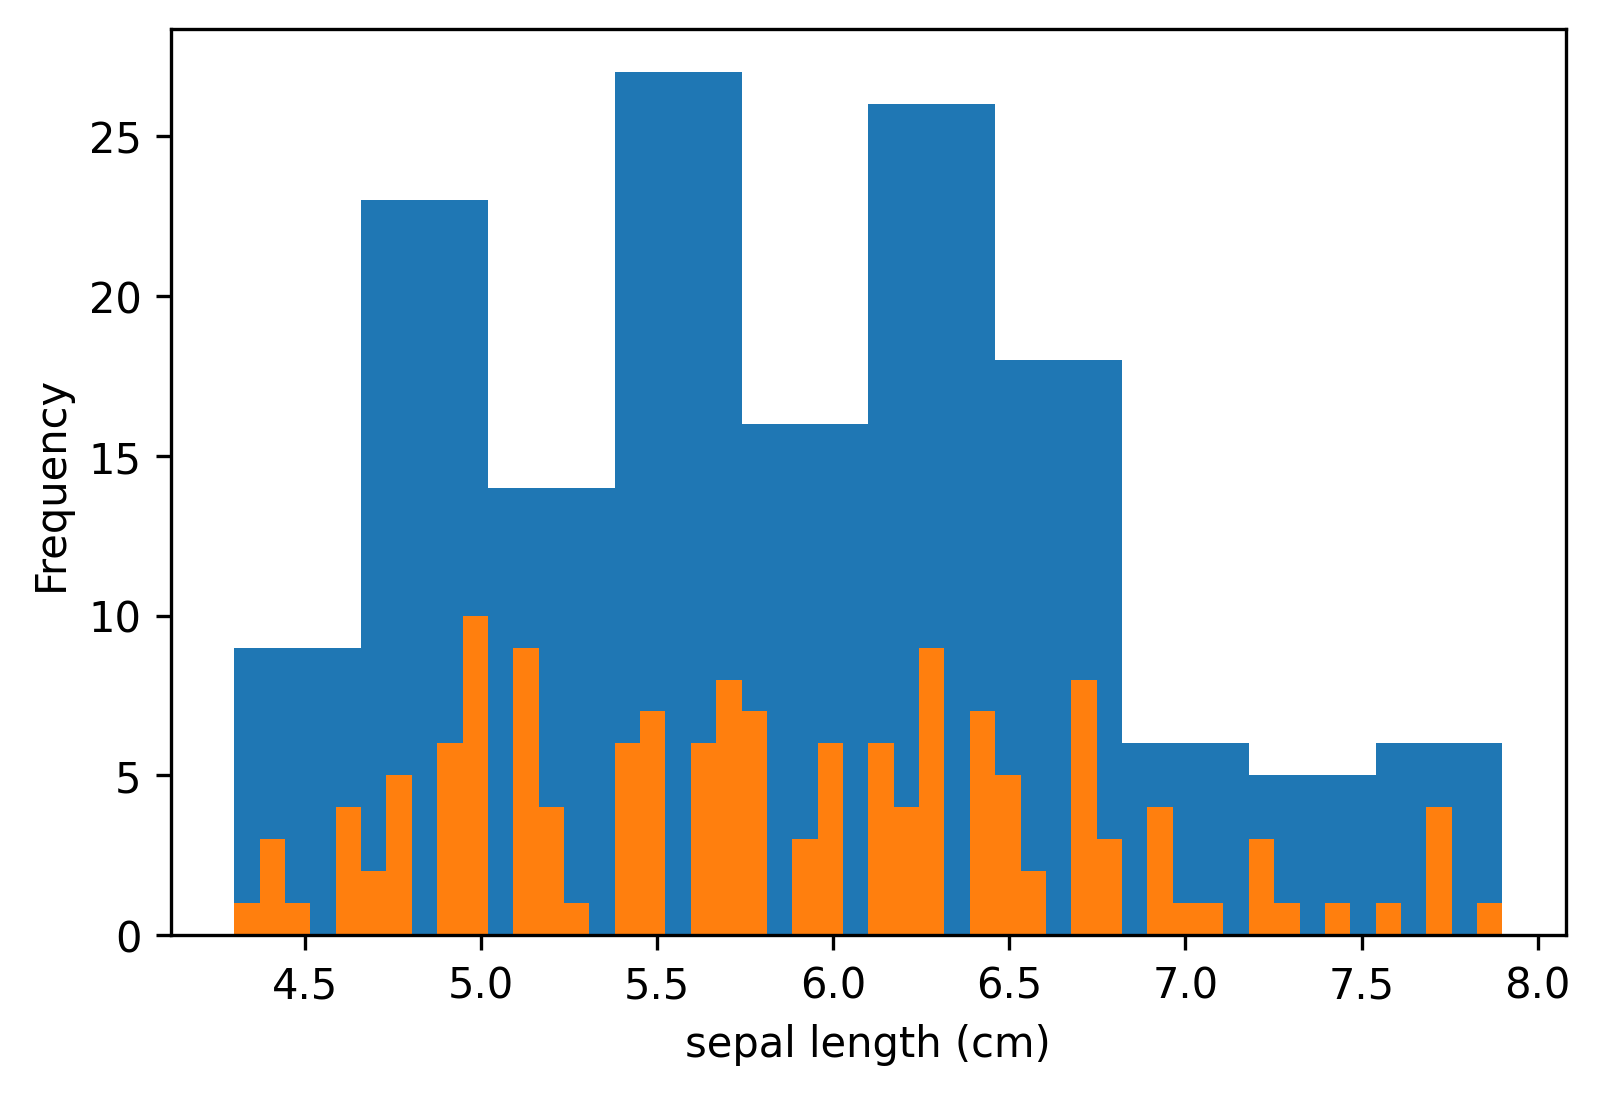
\includegraphics[width=.6\textwidth]{./figure/hist_iris_sepal_length.png}
                      
                      empirical cumulative density function (eCDF)\\
                      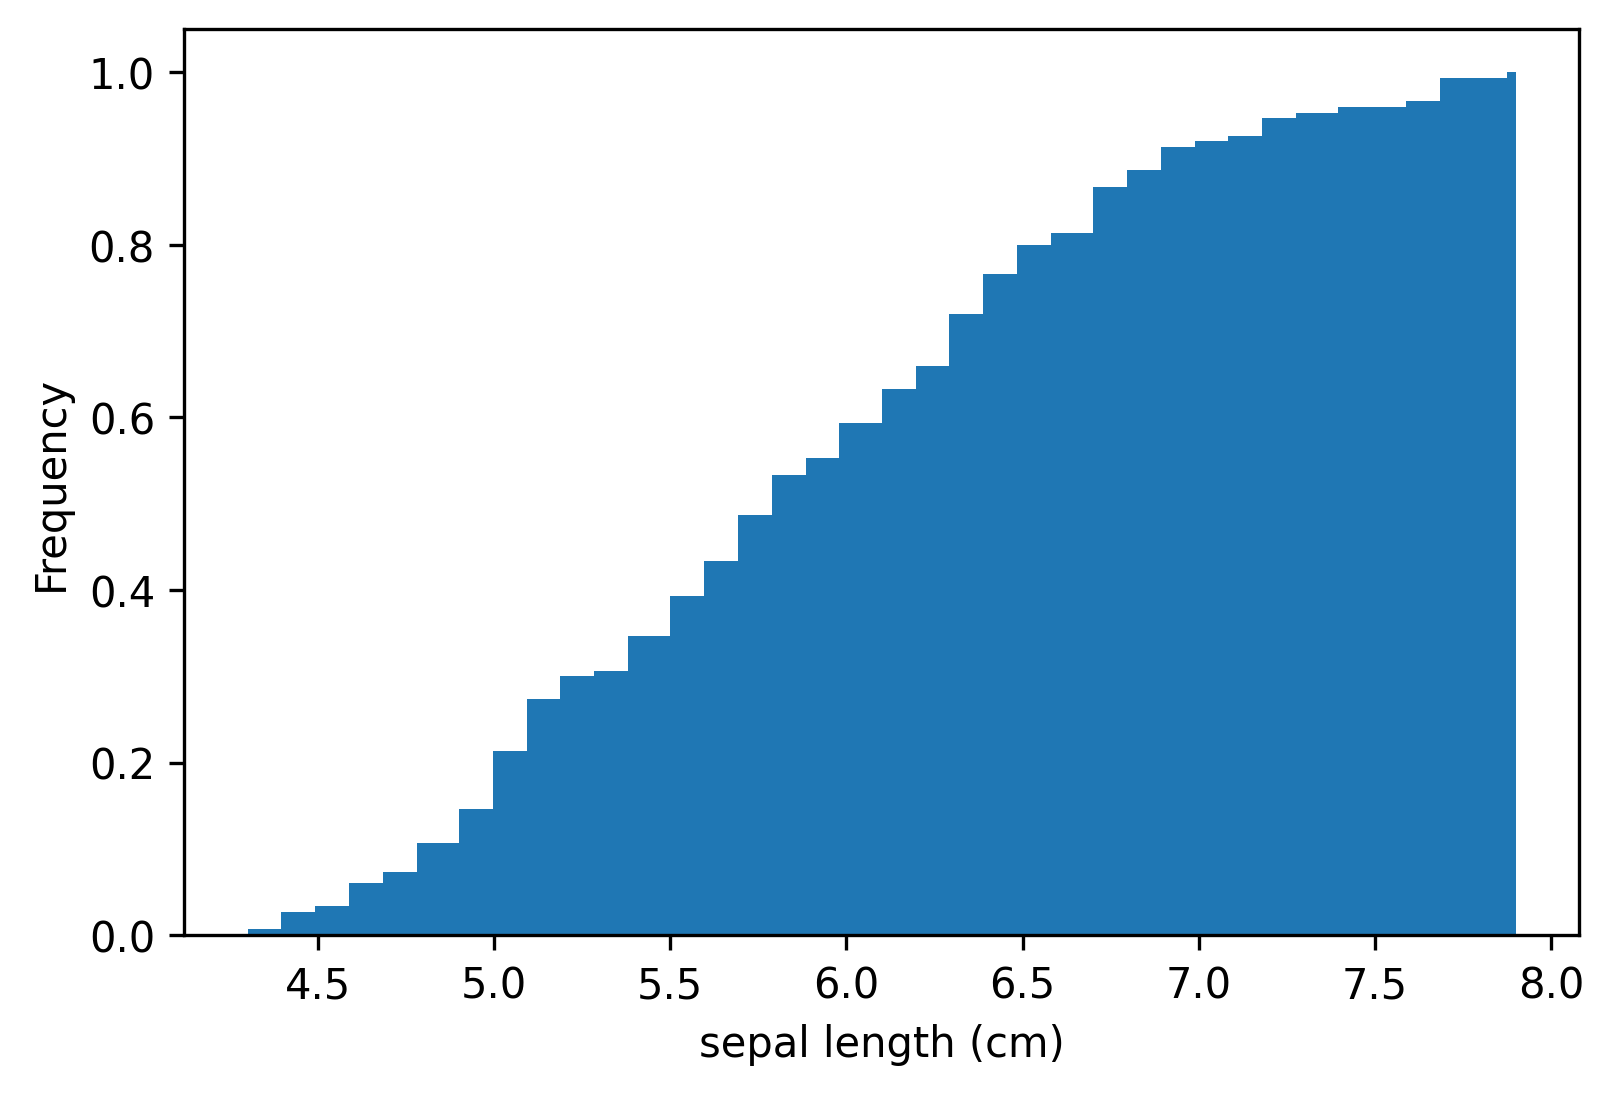
\includegraphics[width=.6\textwidth]{./figure/cdf_iris_sepal_length.png}
            \end{column}
            
            \begin{column}{.5\textwidth}
            
                \begin{itemize}
                    \item Both plot the same data\\ (i.e., sepal length of the iris dataset)
                    \item eCDF does not depend on the number of bins
                    \item eCDF reveals the median (and all other percentiles \& quartiles)
                    \item Based on the shape of eCDF, you can find probability mass
                \end{itemize}

            \end{column}
        \end{columns}
    \end{frame}
    
    
    \begin{frame}{Density curves}
        \begin{columns}
            \begin{column}{.4\textwidth}
            
                      \centering
                      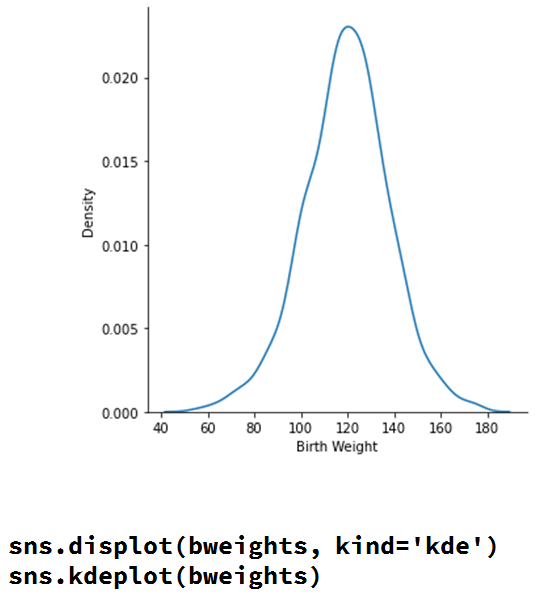
\includegraphics[scale=.3]{Bild33}

                sns.displot(bweights, kind='kde')\\
                sns.kdeplot(bweights

            \end{column}
            
            
            \begin{column}{.6\textwidth}

                  We can also plot a density curve by itself, by appropriately setting the parameters of sns.displot or calling directly sns.kdeplot.\\
                %\bigskip
                %In the next lecture, we will study how exactly to compute these density curves (using a technique is called Kernel Density Estimation). \\
                %\bigskip
                %With the appropriate parameter, we can also add a rug plot to our density curve.

            \end{column}
        \end{columns}
    \end{frame}
\end{document}